\chapter{Performance Evaluation}
\section{Experiment Setup}
\label{sec:evaluation:setup}
In this chapter, we present the performance evaluation of DeAr and demonstrate its capability of efficient arithmetic.
Two benchmark suites were prepared for the experiment.
The first one is adapted from the BLAS~\cite{blas} library, 
which contains various matrix arithmetic subprograms that are crucial in wireless communication.
The second one include general DSP kernels (GDSPK) selected from classic DSP benchmark suites, BDTI~\cite{bdti} and DSPstone~\cite{dspstone}.
Table~\ref{tab:op} lists the operation profiling of two benchmark suites, 
where each subprogram/kernel comprises three primitive operations, addition, multiplication and shifting.
\begin{table}[!ht]
    \centering
    \caption{Operation profiling of two benchmark suites}
    \label{tab:op}
    \resizebox{\columnwidth}{!}
    {
        \begin{tabular}{|c|c|c|c|c|c|c|c|c|}
            \hline
            \multicolumn{9}{|c|}{\textbf{Basic linear algebra subprograms (BLAS)}} \\ \hline
            Benchmark              & AXPY   & MV     & MM      & INV      & CAXPY  & CMV  & CMM    & CINV  \\ \hline
            \# add            &  32    &  56    &   48    &    75    &  128   & 132  &   90   &  88   \\ \hline
            \# mul            &  32    &  64    &   64    &   172    &  128   & 144  &  108   & 114   \\ \hline
            \# sht            &   0    &   0    &    0    &     0    &    0   &   0  &    0   &   0   \\ \hline
            \# op             &  64    & 120    &  112    &   247    &  256   & 276  &  198   & 202   \\ \hline
            \multicolumn{9}{|c|}{\textbf{General DSP kernels (GDSPK)}}                     \\ \hline
            Benchmark              & FIR    & CFIR   & LPFIR   & Biquad   & IT     & DCT  & IMDCT  & FFT   \\ \hline
            \# add            & 15     &  62    &   15    &    8     &  32    &  29  &   21   &  23   \\ \hline
            \# mul            & 16     &  64    &    8    &    9     &   0    &  12  &   11   &  10   \\ \hline
            \# sht            &  0     &   0    &    0    &    0     &  10    &   9  &    9   &   0   \\ \hline
            \# op             & 31     & 126    &   23    &   17     &  42    &  50  &   41   &  33   \\ \hline
        \end{tabular}
    }
\end{table}
\\\indent Figure~\ref{fig:sim} shows the simulation environment of the experiment, 
where DeAr, scalar, VLIW, and composite-ALU architectures \cite{cascade} were evaluated for comparison. 
The instruction unit provided stimulus to the design under test (DUT) from IM,
and the L/S unit handled data between the DUT and DM.
The DUT was replaced in accordance with DeAr and other architectures, 
which had identical ALU composed one adder, one multiplier and one shifter.
Note that we selected best two ALU orders, M-S-A and A-M-S, to implement the composite-ALU architecture.
Please refer to Figure~\ref{fig:vliw} and \ref{fig:cascade} for details of the VLIW and composite-ALU architectures.
\vspace{\textfig}
\begin{figure}[!ht] 
    \centering
    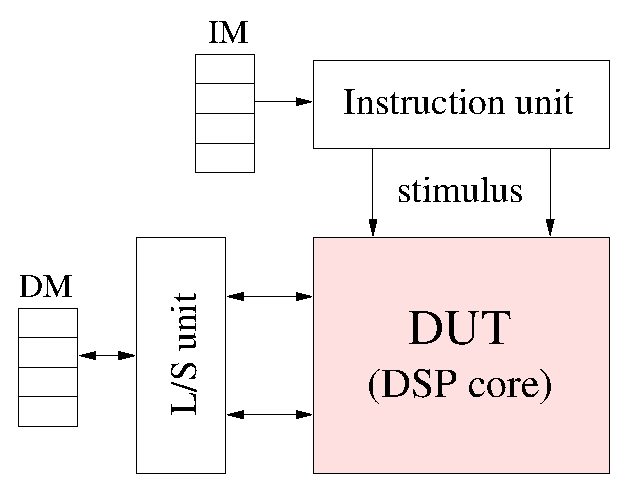
\includegraphics[width=0.6\textwidth]{./figs/sim.eps}
    \caption{Simulation environment}
    \label{fig:sim}
\end{figure}
\\\indent It is important to note that we focused on single-core architectures instead of the multi-core ones in the experiment.
Currently, benchmark results of multi-core systems are highly correlated with the amount of optimization applied to the interconnection and the memory subsystem~\cite{trends}.
Moreover, the programming language also plays a crucial role in multi-core system performance, 
but popular ones such as CUDA, OpenCL and OpenMP are still contending for adoption as the industry standard.
Consequently, the development of a fair benchmark suiting for multi-core DSP platforms is still an open field of study~\cite{landscape}.
Owing to aforementioned issues, we believe benchmarking the single-core DSPs can present more objective evaluation, 
Note that the implementation of VLIW and 
\section{Pre-synthesis Analysis}
{
    \subsection{Operations per Cycle}
    Operations per cycle (OPC) evaluates the utilization rate of the ALU.
    This metric wsa obtained by statically scheduling operations of a DSP kernel for various architectures.
    Under the performance requirement of target applications, OPC helps to determine the timing constraint for hardware synthesis, 
    where higher OPC brings looser timing constraint, which results in lower cost from the post-synthesis hardware.
    Table~\ref{tab:opc} profiles the OPC of the DSP cores with the assumption that every operation consumes exactly one clock cycle.
    \\\indent The OPC of the scalar processor was fixed to 1.0 because of the limitation of the single-issue datapath.
    On the contrary, benefiting from the wide issue-width and large port number of RF, VLIW gained the best OPC in all benchmarks.
    %Looking into the issue-width of VLIW, 
    %the 3-way configuration only brought little advantages, 0\% and 1.82\% respectively in two benchmark suites, over the 2-way configuration because of sparsity of shift operations.
    The OPC of DeAr was limited by the access pattern of the sequential-access banked RF, which either be LIFO or FIFO, 
    and thus it was not possible for DeAr to out-perform the VLIW in regard to OPC.
    Nevertheless, by leveraging the novel scheduling algorithm in \ref{sec:scheduling},  
    DeAr still gained approximate OPC of the VLIW, with only 1.11\% and 4.26\% loss two benchmark suites.
    On the other hand, the OPC of composite FU architecture is highly correlated with the cascade order and the benchmark characteristic. 
    On average, the MSA order gains better OPC than the AMS order, 
    but the former still underperformed 3-way VLIW by 12.3\% and 17.7\% in the benchmarks suites.
    \begin{table}[!ht]
        \centering
        \caption{Operations per cycle profiling}
        \label{tab:opc}
        \resizebox{\columnwidth}{!}
        {
            \begin{tabular}{|c|c|c|c|c|c|c|c|c|c|}
                \hline
                \multicolumn{10}{|c|}{\textbf{Basic linear algebra subprograms (BLAS)}} \\ \hline
                Benchmark  &  AXPY  &  MV  &  MM  &  MINV  &  CAXPY  &  CMV  &  CMM  &  CMINV  &  Average \\ \hline 
                VLIW  &   1.94  &   1.85  &   1.72  &   1.44  &   1.97  &   1.89  &   1.80  &   1.76  &   1.79     \\ \hline 
                %2-way VLIW  &   1.94  &   1.85  &   1.72  &   1.44  &   1.97  &   1.89  &   1.80  &   1.76  &   1.79     \\ \hline 
                DeAr  &   1.94  &   1.85  &   1.72  &   1.40  &   1.97  &   1.89  &   1.80  &   1.62  &   1.77     \\ \hline
                Composite-MSA  &   2.00  &   1.88  &   1.75  &   1.37  &   1.33  &   1.35  &   1.38  &   1.53  &   1.57     \\ \hline 
                Composite-AMS  &   1.00  &   1.00  &   1.00  &   1.02  &   1.00  &   1.00  &   1.00  &   1.04  &   1.01     \\ \hline 
                Scalar  & 1.0  & 1.0  & 1.0  & 1.0  & 1.0  & 1.0  & 1.0  & 1.0  & 1.0 \\ \hline 
                \multicolumn{10}{|c|}{\textbf{General DSP application kernels (GDSPK)}}                     \\ \hline
                Benchmark  &  FIR  &  CFIR  &  LPFIR  &  Biquad  &  IT  &  DCT  &  IMDCT  &  FFT  &  Average \\ \hline 
                VLIW  &   1.82  &   1.91  &   1.67  &   1.55  &   1.33  &   1.61  &   1.86  &   1.38  &   1.64     \\ \hline 
                %2-way VLIW  &   1.82  &   1.91  &   1.67  &   1.55  &   1.33  &   1.56  &   1.64  &   1.38  &   1.61     \\ \hline 
                %         ^fix 1.67 to 1.82              ^fix 1.42 to 1.54                                 ^ fix 1.61 to 1.62
                DeAr  &   1.82  &   1.91  &   1.67  &   1.55  &   1.33  &   1.47  &   1.46  &   1.32  &   1.57     \\ \hline 
                Composite-MSA  &   1.94  &   1.34  &   1.44  &   1.42  &   1.31  &   1.14  &   1.28  &   1.06  &   1.35     \\ \hline 
                Composite-AMS  &   1.00  &   1.00  &   1.53  &   1.21  &   1.14  &   1.61  &   1.52  &   1.27  &   1.29     \\ \hline 
                Scalar  & 1.0  & 1.0  & 1.0  & 1.0  & 1.0  & 1.0  & 1.0  & 1.0  & 1.0 \\ \hline 
            \end{tabular}
        }
    \end{table}
    \subsection{Register file access rate}
    Register file access rate provides a quantitative measurement of the register file activity, 
    which makes up the majority of power dissipation in DSP cores.
    It is calculated dividing the real number of register file accesses by the worst case number of accesses.
    Table~\ref{tab:rpd} profiles the RF access rate of each architecture in regard to various benchmarks.
    Under the assumption of single cycle datapaths, conventional architectures, scalar and VLIW, 
    lack bypassing capability and write back arithmetic results every cycle, 
    We referred to such a scenario as the worst case in regard to RF access, 
    and thus their RF access rate is fixed to 1.0.
    On the contrary, DeAr leveraged TTDB and HDFG-based scheduling to explore data bypassing opportunities. 
    As a result, its RF access rate was reduced to 0.69 and 0.73, 
    and out-performed the best composite order, MSA, which had the RF access rate of 0.77 and 0.82 respectively in two benchmark suites.
    \begin{table}[!ht]
        \centering
        \caption{Register file access rate profiling}
        \label{tab:rpd}
        \resizebox{\columnwidth}{!}
        {
            \begin{tabular}{|c|c|c|c|c|c|c|c|c|c|}
                \hline
                \multicolumn{10}{|c|}{\textbf{Basic linear algebra subprograms (BLAS)}} \\ \hline
                Benchmark  &  AXPY  &  MV  &  MM  &  MINV  &  CAXPY  &  CMV  &  CMM  &  CMINV  &  Average \\ \hline 
                DeAr  &   0.67  &   0.69  &   0.71  &   0.67  &   0.67  &   0.68  &   0.70  &   0.71  &   0.69     \\ \hline
                Composite-MSA  &   0.67  &   0.69  &  0.71  &   0.82  &   0.83  &   0.83  &   0.82  &   0.77  &  0.77     \\ \hline 
                Composite-AMS  &   1.0  &   1.00  &   1.00  &   0.98  &   1.00  &   1.00  &   1.00  &   0.97  &   0.99     \\ \hline 
                VLIW  &   1.00  &   1.00  &   1.00  &   1.00  &   1.00  &   1.00  &   1.00  &   1.00  &   1.00     \\ \hline 
                %2-way VLIW  &   1.00  &   1.00  &   1.00  &   1.00  &   1.00  &   1.00  &   1.00  &   1.00  &   1.00     \\ \hline 
                Saclar  &   1.00  &   1.00  &   1.00  &   1.00  &   1.00  &   1.00  &   1.00  &   1.00  &   1.00     \\ \hline 
                \multicolumn{10}{|c|}{\textbf{General DSP kernels (GDSPK)}}                     \\ \hline
                Benchmark  &  FIR  &  CFIR  &  LPFIR  &  Biquad  &  IT  &  DCT  &  IMDCT  &  FFT  &  Average \\ \hline 
                DeAr  &   0.68  &   0.67  &  0.60  &   0.57  &   0.85  &   0.74  &   0.86  &   0.82  &   0.73     \\ \hline 
                Composite-MSA  &   0.68  &   0.83  &   0.80  &   0.80  &   0.83  &   0.87  &   0.80  &   0.92  &   0.82     \\ \hline 
                Composite-AMS  &   1.00  &   1.00  &   0.77  &   0.88  &   1.00  &   0.76  &   0.84  &   0.86  &   0.87     \\ \hline 
                VLIW  &   1.00  &   1.00  &   1.00  &   1.00  &   1.00  &   1.00  &   1.00  &   1.00  &   1.00     \\ \hline 
                %2-way VLIW  &   1.00  &   1.00  &   1.00  &   1.00  &   1.00  &   1.00  &   1.00  &   1.00  &   1.00     \\ \hline 
                Saclar  &   1.00  &   1.00  &   1.00  &   1.00  &   1.00  &   1.00  &   1.00  &   1.00  &   1.00     \\ \hline 
            \end{tabular}
        }
    \end{table}
    %\subsection{Code size}
    %To evaluate code size fairly, we defined a new metric, effective instruction width (EIW), 
    %which normalize code size with OPC.
    %We calculated EIW by dividing the instruction issue-width by the averaged OPC of two benchmark suites in Table~\ref{tab:opc}, 
    %We assumed that the total number of registers in the RF is 32, 
    %which implies 5 bits are needed to address the centralized RF, 
    %as well as that each architecture uses 4 bits for function selection and 5 bits for specifying shift amount.
    %Table~\ref{tab:density} shows the EIW of each architecture.
    %Benefiting from implicit RF access, DeAr achieved the lowest EIW, which was only 64.3\% and 43.5\% of the 2-way and 3-way VLIW.
    %By reducing the number of operands to be specified, the composite-ALU architecture achieved the EIW in between DeAr and the scalar.
    %On the other hand, since the averaged OPC could not grow linearly with the issue-width, 
    %the VLIW obtained worse and worse EIW than the scalar as the issue-width increased.
    %\begin{table}[!ht]
    %    \centering
    %    \caption{Code size evaluation by EIW}
    %    \label{tab:density}
    %    \resizebox{\columnwidth}{!}
    %    {
    %        \begin{tabular}{|c|c|c|c|c|c|c|}
    %            \hline
    %            & DeAr & Composite-MSA  & Composite-AMS  & Scalar & 2-way VLIW & 3-way VLIW \\ \hline
    %            Issue-width        & 24   & 28   & 28   & 19     & 38    & 57    \\ \hline
    %            Averaged OPC       & 1.67 & 1.46 & 1.15 & 1.0    & 1.70  & 1.72  \\ \hline
    %            EIW                & 14.4 & 19.2 & 25.2 & 19     & 22.4  & 33.1  \\ \hline
    %        \end{tabular}
    %    }
    %\end{table}
}
\section{Synthesis Result and Analysis}
{
    In this section, we present hardware synthesis results with target throughput varying from 50 to 1000 MOPS, 
    We implemented aforementioned designs with UMC 65nm cell library, 
    and measured their area and power dissipation with Synopsys Design Compiler and Synopsys Prime Time under the throughput constraint based on Table~\ref{tab:opc}.
    Synthesis failures owing to timing violation reported by the tool would remain their entries empty in figures.
    \subsection{Area}
    Figure~\ref{chart:area} shows the synthesis area of DSP cores regarding to the BLAS (a) and GDSPK (b) benchmark suites.
    The proposed DeAr saved 24.5\%--21.1\% and 24.9\%--21.6\% of area in BLAS and GDSPK respectively compared with VLIW.
    %When compared with 3-way VLIW, the saved percentage further increased to 35.4\%--31.7\% (BLAS) and 35.2\%--31.1\% (GDSPK).
    The area of the VLIW architecture were dominated by RF, 
    which demanded complicated interconnection among ports and registers to facilitate centralized organization.
    By contrast, DeAr, which traded of the connectivity by adopting the banked RF, could thus achieve significant area reduction.
    Since RF access was not the crucial issue affecting the critical path for both VLIW and DeAr, 
    the correlation between throughput and saved percentage was inconspicuous.
    \\\indent On the other hand, DeAr achieved 21.2\%--5.6\% (BLAS) and 33.5\%--4.8\% (GDSPK) area reduction against composite-ALU with the MSA order.
    When compared with the AMS order, the saved percentage became 17.2\%--5.3\% (BLAS) and 10.5\%--4.7\% (GDSPK).
    Composite-ALU architectures reduced area by using fewer ports on the RF.
    Nevertheless, the area burden caused by the centralized RF still existed.
    Another drawback of composite-ALU architectures is long critical path in the ALU, 
    which leaded to exploding area growth when throughput increasing.
    \\\indent Benefiting from the simplicity of the datapath, 
    the scalar costed lowest area when target throughput was low.
    However, the low OPC of scalar became the terrible burden on achieving high throughput.
    The area of scalar exceeded the one of DeAr as throughput was above 600 MOPS (BLAS) or 650 MOPS (GDSPK).
    Consequently, DeAr achieved lowest area among six designs when throughput is high.
    \vspace{\textfig}
    \begin{figure}[!ht]
        \begin{center}
            \subfigure[BLAS benchmark suite]
            {
                \label{chart:area:blas}
                \includegraphics[width=0.48\textwidth]{charts/area_blas.eps}
            }
            \subfigure[General benchmark suite]
            {
                \label{chart:area:general}
                \includegraphics[width=0.48\textwidth]{charts/area_general.eps}
            }
        \end{center}
        \caption{Synthesis area of the DSP cores}
        \label{chart:area}
    \end{figure}

    \subsection{Power dissipation}
    The power dissipation in CMOS devices is constituted by dynamic power and static power.
    In our experiment, the former was the dominating factor, which accounted for X-Y\% of the total dissipation, 
    owing to the cell library characteristic, 
    As a result, our analysis focused on the dynamic power, 
    which is proportional to the product of clock rate $f$, logic switching rate $\alpha$ and the load $C_L$ of each cell.
    \\\indent
    Figure~\ref{chart:area} shows the power dissipation of each DSP core, 
    which grew near-linearly with throughput and various slope.
    DeAr saved 22.7\%--15.1\% (BLAS) and 18.5\%--10.4\% (GDSPK) of power compared with the VLIW.
    %and 21.1\%--16.5\% (BLAS) and 17.3\%--13.1\% (GDSPK) of power compared with the 3-way VLIW.
    The power reduction achieved by DeAr was attributed to its low register access rate, which reduced $\alpha$
    and banked RF organization, which reduced $C_L$, in the RF.
    \\\indent
    The power dissipation of composite-ALU was significantly affected by ALU order.
    Below 600 MOPS, DeAr achieved 46.9\%--41.2\% (BLAS) and 19.7\%--15.8\% (GDSPK) power reduction against AMS, 
    but only achieved 7.1\%--2.6\% (BLAS) and 11.4\%--1.5\% (GDSPK) against MSA.  Compared with AMS, MSA benefited from high OPC, which reduced $f$, and low RF access rate, which reduced $\alpha$, 
    so it could stay competitive against DeAr in this metric.
    However, the exploding area growth of composite-ALU led to significant growth of $C_L$ in the long run.
    As a result, power dissipation of MSA gradually diverged from the one of DeAr as throughput increasing, 
    and DeAr achieved 22.5\%--8.7\% (BLAS) and 37.8\%--12.1\% (GDSPK) reduction against MSA when throughput was above or equal 600 MOPS, 
    where the synthesis for AMS failed.
    \\\indent
    Although the scalar processor cost low area, which implies low $C_L$, 
    the worst OPC and RF access rate among designs brought unfavorable $f$ and $\alpha$, 
    which resulted in severe power dissipation. 
    Compared with the scalar, DeAr saved 52.1\%--45.8\% (BLAS) and X1-Y1\% (GDSPK) of power below 700 MOPS, 
    and the synthesis for scalar failed above 700 MOPS.
    In regard to power dissipation, DeAr achieved the best result among designs regardless throughput.
    \vspace{\textfig}
    \begin{figure}[!ht]
        \begin{center}
            \subfigure[BLAS benchmark suite]
            {
                \label{chart:power:blas}
                \includegraphics[width=0.48\textwidth]{charts/power_blas.eps}
            }
            \subfigure[General benchmark suite]
            {
                \label{chart:power:general}
                \includegraphics[width=0.48\textwidth]{charts/power_general.eps}
            }
        \end{center}
        \caption{Power dissipation of the DSP cores}
        \label{chart:area}
    \end{figure}

    %\subsection{Leakage Power Dissipation}
    %\vspace{\textfig}
    %\begin{figure}[!ht]
    %    \begin{center}
    %        \subfigure[BLAS benchmark suite]
    %        {
    %            \label{chart:leakage:blas}
    %            \includegraphics[width=0.48\textwidth]{charts/leakage_blas.eps}
    %        }
    %        \subfigure[General benchmark suite]
    %        {
    %            \label{chart:leakage:general}
    %            \includegraphics[width=0.48\textwidth]{charts/leakage_general.eps}
    %        }
    %    \end{center}
    %    \caption{Leakage power dissipation of DSP cores}
    %    \label{chart:leakage}
    %\end{figure}
}


